% !TEX root =  master.tex
\section{Implementierung des Saalplans}

Eine zentrale Aufgabe im Front-End war es, den Kinosaal mit den Sitzen anzuzeigen und dem Benutzer zu ermöglichen, Plätze auszuwählen.

Dies lässt sich mit einfachen Mitteln auch in \acs{HTML} umsetzen, z.B. mit \textit{div}-Elementen, bei denen man Größe und Farbe festlegt.
Mit JavaScript wird dann implementiert, was passiert wenn ein Sitzplatz angeklickt wird.

In der Abbildung \vref{fig:saalplan01} kann man sehen, wie der Kinosaal im Browser dargestellt wird.
Eine Box außen bildet die Umrandung und stellt den Saal dar.
Darin befindet sich eine zweite farblich hervorgehobene Box, die die Leinwand abbildet, damit die Benutzer wissen, wo im Kinosaal vorne und hinten ist, und sie somit ihre Entscheidung, wo sie sitzen möchten, treffen können.
Darunter finden sich dann die Sitzplätze.

\begin{figure}[ht]
	\centering
	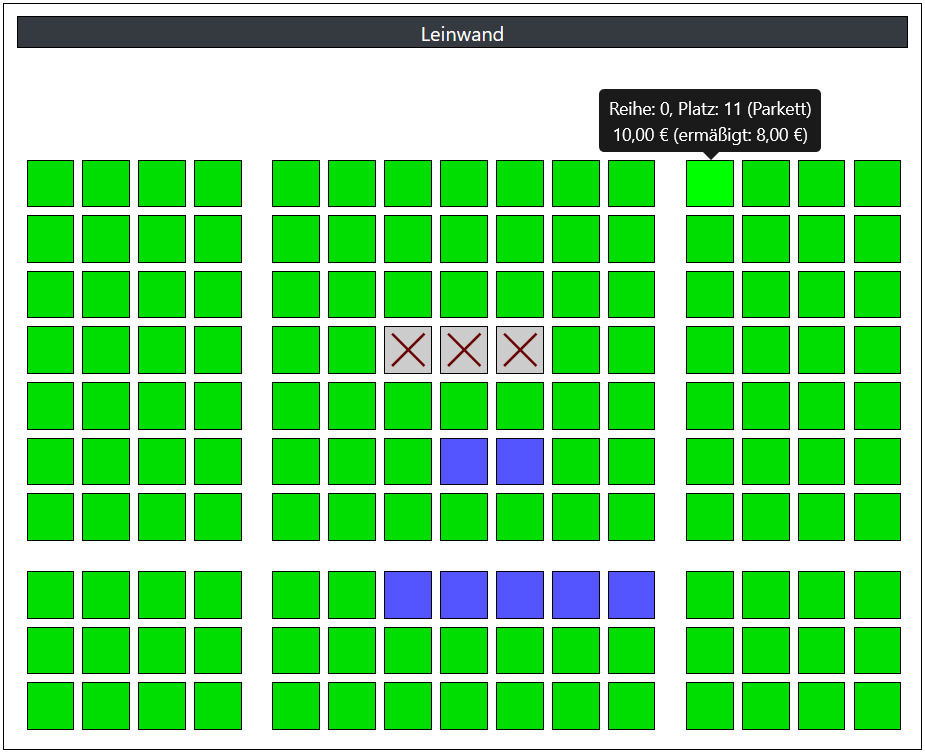
\includegraphics[width=0.8\textwidth]{img/screenshots/saalplan01}
	\captionsetup{format=hang}
	\caption{\label{fig:saalplan01}Saalplan}
\end{figure}

Die Sitzplätze sind dabei farblich gekennzeichnet, um anzuzeigen, ob ein Sitzplatz frei oder belegt ist.
Belegte Sitze sind einerseits grau, andererseits auch noch mit einem Kreuz versehen, um Menschen, die in ihrer Farbwahrnehmung eingeschränkt sind, zu berücksichtigen.
Außerdem werden ausgewählte Sitze blau markiert und der Sitz, über dem aktuell die Maus ist, wird ebenso hervorgehoben.
Ein Tooltip mit einer kurzen Beschreibung und Details zu Kategorie und Preis, gibt dem Benutzer weitere Informationen.

Das Aussehen der Sitzplätze wird über Klassen und eine eigene \acs{CSS}-Datei definiert, sodass sich dies schnell anpassen lässt und zum Beispiel die Farbe der Sitzplätze mit einem Mal änderbar ist.

\begin{figure}[ht]
	\centering
	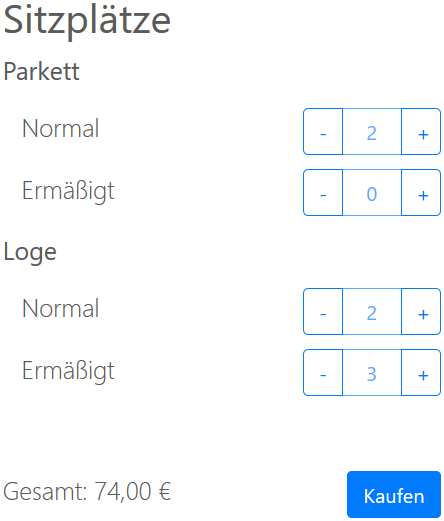
\includegraphics[width=0.4\textwidth]{img/screenshots/saalplan02}
	\captionsetup{format=hang}
	\caption{\label{fig:saalplan02}Preisstufen}
\end{figure}

Wählt man nun Sitzplätze aus, so muss man noch angeben, wie viele Tickets zum normalen Preis man kaufen möchte und wie viele zu einem ermäßigten Preis.
Daraus wird dann direkt der Preis berechnet und angezeigt.
Je nach Bildschirmgröße und -dimensionen werden diese Element neben dem Saalplan oder darunter angezeigt.
Mit dem \enquote{Kaufen}-Button gelangt man dann zur nächsten Seite, um weitere Daten anzugeben.

In der ersten Implementierung wurden der Saal und die Sitzplätze mit absoluten Größenangaben definiert.
So hatte das \textit{div}-Element, das einen Sitzplatz darstellt, als Höhe und Breite \textit{20px} gesetzt und eine Position relativ zur links oberen Ecke des Saals in Pixeln angegeben.
Die Koordinaten kommen dabei direkt aus dem Back-End bzw. der Datenbank.
Dies ermöglicht es, nicht nur einfach alle Plätze nebeneinander anzuzeigen, sondern auch Gänge einzufügen, Plätze versetzt anzuordnen, die Abstände zwischen den Sitzen individuell zu gestalten und somit den Saalplan an die Realität anzupassen.

\begin{figure}[ht]
	\centering
	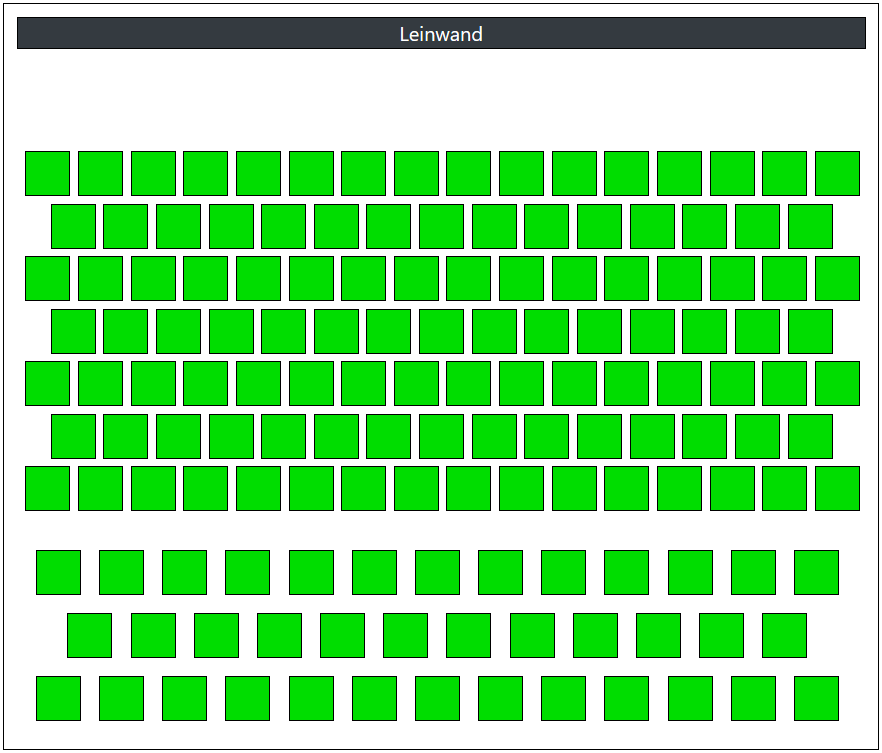
\includegraphics[width=0.8\textwidth]{img/screenshots/saalplan03}
	\captionsetup{format=hang}
	\caption{\label{fig:saalplan03}Saalplan}
\end{figure}
